\section{Operational Context and Trust Foundations}

\subsection{A Heterogeneous Mission System of Systems}

The core system contains UAVs, USVs, and UUVs that contribute different sensing, mobility, computation, and communications functions. UAVs offer rapid repositioning, line-of-sight radio relays, and electro-optical sensing, but their payload, endurance, and link stability are constrained. USVs can carry larger energy stores and antennas, remain on station, and bridge acoustic and radio networks. UUVs provide proximity to underwater targets and environments but frequently depend on low-rate acoustic channels, short-range optical links, or delayed surfacing for high-volume transfer. Surveys of UAV-aided maritime communication and 6G maritime connectivity illustrate the relay opportunities \citep{nomikos2023survey,nomikos2024improving}; underwater communication reviews document the trade-offs among acoustic, optical, and other media \citep{ali2020recent,saeed2019underwater,diamant2018low,jahanbakht2021internet}. The resulting system requires a dynamic network model in which topology, latency, bandwidth, clock quality, and reachability can change during a single mission.

Full-text inspection sharpens this point. Civil-UAV communication requirements are explicitly mission-dependent: application classes vary in network role, data volume, range, and quality-of-service needs \citep{hayat2016survey}. Maritime-search evidence characterizes heterogeneous cooperative systems as an early-stage applied field built on increasingly mature UAV, USV, and UUV capabilities \citep{li2023survey}. Mission trust is therefore conditioned on current role and mission phase, with evidence re-evaluated whenever the application domain or consequence changes.

Cross-domain cooperation also changes fault containment. A USV may be the navigation reference, data cache, radio gateway, and permissioned-ledger peer for several UUVs. Compromise or benign failure of that high-betweenness platform therefore affects link evidence, time, provenance continuity, and access to the shared record. Conversely, platform diversity can improve resilience when evidence from independent media and locations can corroborate an event. Cooperation research demonstrates the control and planning value of heterogeneous formations and multi-swarms \citep{stolfi2021uav,xue2021distributed,liu2023formation,ke2023cross}. Mission assurance extends these results by making the trustworthiness of shared observations, commands, and dependencies explicit.

Administrative heterogeneity is equally important. A civil emergency may combine government responders, commercial communications providers, research vehicles, and contracted data services. A coalition mission may include platforms that remain under distinct authorities. Cross-organizational authority therefore combines local authentication with policy equivalence, delegated roles, and accountable governance. The system boundary includes organizations, credentials, data-use restrictions, software and model versions, and the process that admits, suspends, or removes participants. Under these conditions, a shared ledger can provide a consistent audit state whose history is jointly governed by the participating parties.

\begin{figure}[H]
\centering
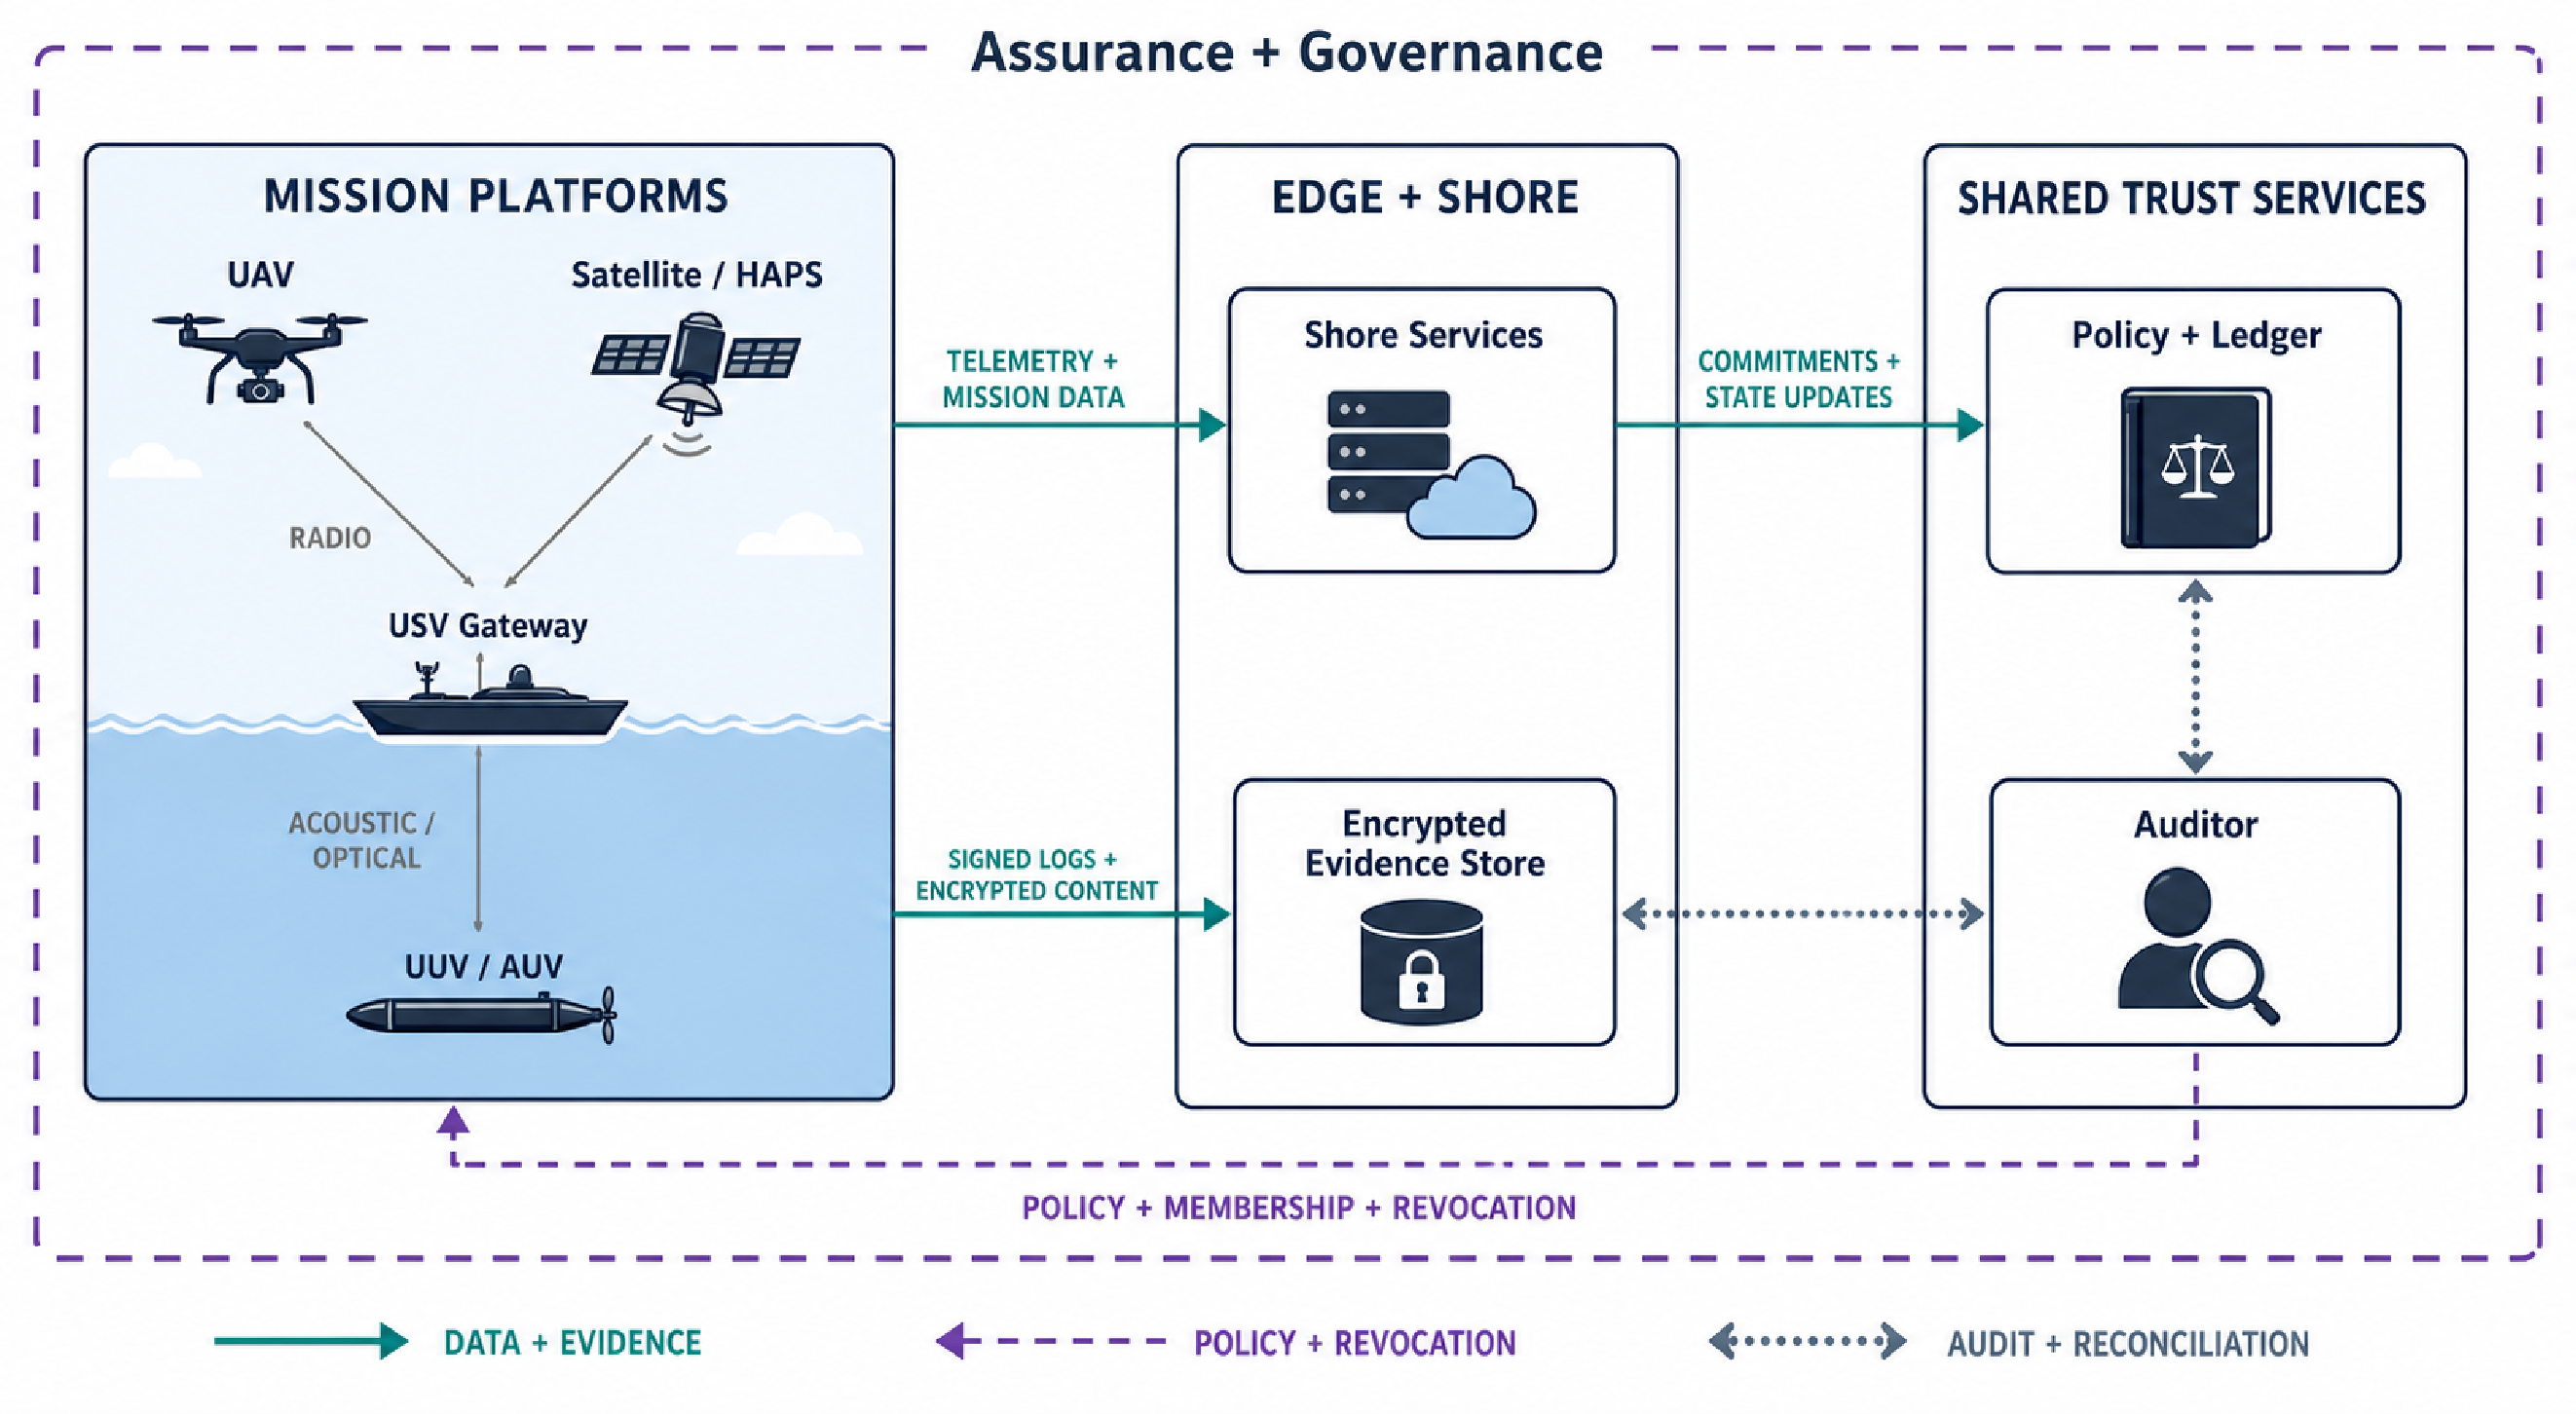
\includegraphics[width=\textwidth]{figures/figure-01-reference-architecture.pdf}
\caption{Author-proposed cross-domain reference architecture. Solid teal arrows show data and evidence moving toward shore and shared services; dashed violet arrows show policy, membership, and revocation returning to mission platforms; dotted slate links show audit and reconciliation. Radio and acoustic/optical media are labeled on neutral topology lines. Constrained platforms retain signed local logs, while capable gateways and shore services forward commitments when connectivity permits. The dashed enclosure identifies the cross-cutting assurance and governance plane.\label{fig:architecture}}
\end{figure}

Figure~\ref{fig:architecture} presents an adaptable logical deployment. Raw imagery, sonar, telemetry, and detailed attestations remain encrypted off chain. A permissioned ledger may retain content identifiers, commitments, coarse-grained state transitions, membership changes, policy and model versions, revocations, and audit decisions. During disconnection, an edge node keeps an append-only signed sequence and later submits a batch commitment. Reconciliation reveals gaps, duplicates, invalid credentials, and conflicting histories; local sensing and control mechanisms retain responsibility for physical interpretation and real-time deadlines.

\subsection{Mission Trust, Trustworthiness, and a Trusted Data Environment}

We define \emph{mission trust} as a context-specific relying decision about whether an object may contribute to a stated mission purpose, given available evidence and the consequences of error. Trust is therefore relational and prospective: a consumer relies on an object for an action. \emph{Trustworthiness} denotes properties that justify such reliance, including identity authenticity, platform integrity, link availability, provenance, freshness, data quality, and accountable governance. Both vary with time and context. The same UAV may be suitable for low-risk environmental imagery while being excluded from time-critical navigation support because its attestation is stale or its location is uncertain.

For an object $o$, time $t$, context $c$, and mission use $m$, a general representation is
\begin{equation}
T_o(t,c,m)=\Pr\!\left(o\text{ satisfies the properties required for }m\mid\mathcal{E}_{1:t},c\right),
\label{eq:trust}
\end{equation}
where $\mathcal{E}_{1:t}$ denotes the direct and indirect evidence currently available. Equation~\eqref{eq:trust} provides a conceptual notation for context-dependent reliance. Implementations may represent the resulting uncertainty through calibrated probabilities, subjective logic, sets, intervals, ordinal states, or decision rules \citep{jsang2016subjective,mui2003computational,kamvar2003eigentrust}. In each representation, uncertainty and evidence lineage remain explicit alongside the trust assessment.

A \emph{trusted data environment} is the socio-technical setting that produces, transports, transforms, shares, and governs evidence and mission data. It includes principals, devices, paths, data products, policies, models, services, and accountability processes. Mission trust is the decision relation exercised within that environment. A tamper-evident catalog strengthens the environment, while mission-use appraisal determines which cataloged item is fit for a particular decision. Zero trust contributes the access-control architecture: NIST's formulation uses policy engines, identity and device evidence, enforcement points, and protected resources \citep{rose2020zero}. Intermittently connected missions add safe degradation and visible evidence staleness to those functions.

\subsection{Four Non-Substitutable Assurance Claims}

The assurance chain in Figure~\ref{fig:assurance-chain} distinguishes four questions. Observation validity asks whether a measurement plausibly represents the physical phenomenon, considering calibration, geometry, environment, sensor health, and corroboration. Commitment and provenance integrity asks who or what produced the item, when and where it was produced, how it was transformed, and whether the recorded bytes and lineage were altered. Ledger and governance consistency asks whether authorized record keepers agree on membership, order, versions, and state transitions under stated fault assumptions. Mission-use suitability asks whether the item is timely, relevant, sufficiently certain, policy-compliant, and proportionate to the consequences of the contemplated action.

\begin{figure}[H]
\centering
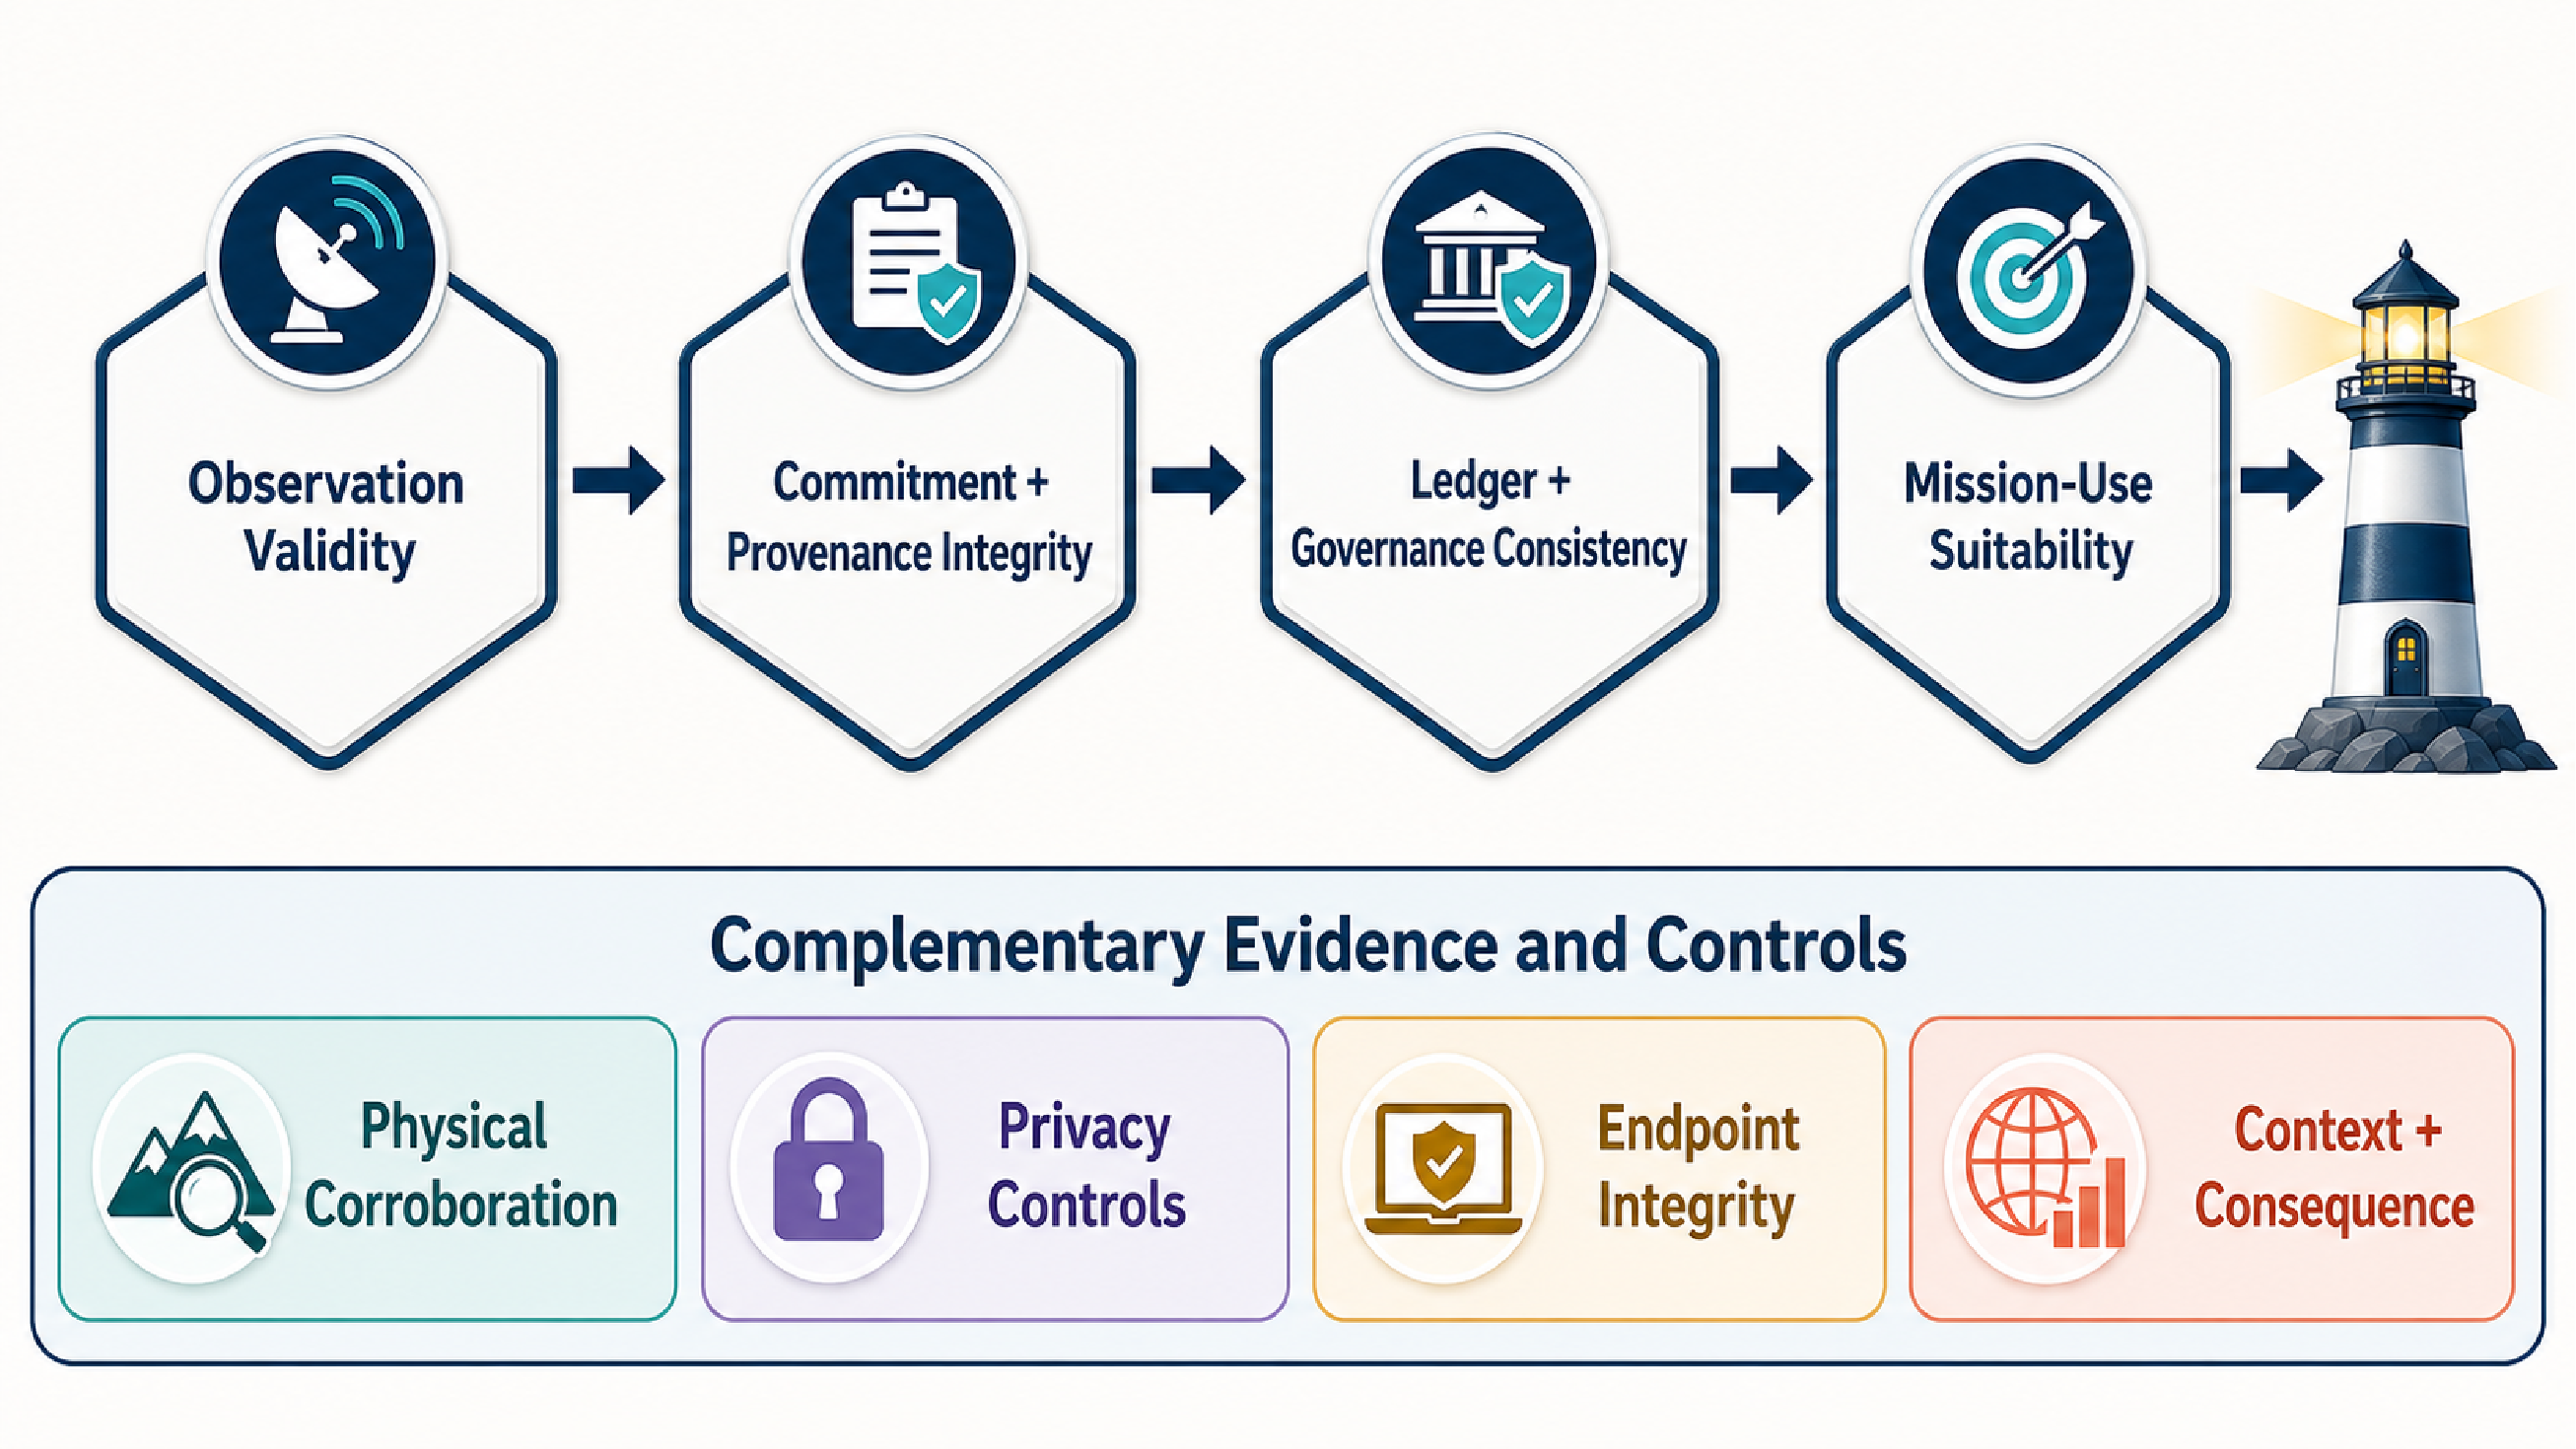
\includegraphics[width=\textwidth]{figures/figure-02-assurance-chain.pdf}
\caption{The authors' four-layer assurance chain. Each layer contributes a distinct claim to the relying decision.\label{fig:assurance-chain}}
\end{figure}

These claims have distinct failure modes. GNSS spoofing can make an otherwise healthy UAV report the wrong location; machine-learning and multi-sensor approaches may detect inconsistency, with validity conditioned on data and context \citep{shafique2021detecting,dang2022deep,semanjski2020use,rado2024recent,varshosaz2019spoofing}. A stolen signing key can produce syntactically valid provenance. A permissioned consensus group can faithfully order false submissions. A delayed but accurate observation can be unfit for collision avoidance. The chain therefore keeps four concepts distinct: signatures and physical truth; hashes and privacy; consensus and endpoint security; and historical reputation and current mission fitness.

Remote attestation and device baselines fit between the first two layers. The RATS architecture distinguishes evidence, appraisal policy, attestation results, and relying parties \citep{birkholz2023remote}; the NIST IoT baseline emphasizes device identification, configuration, data protection, logical access, software update, and cybersecurity-state awareness \citep{fagan2020iot}. These mechanisms justify scoped claims about measured software and device state through roots of trust, reference values, verifier freshness, and explicit measurement coverage. External observation validity is established through complementary physical and sensor evidence. Provenance records derivation: W3C PROV relates entities, activities, and agents, enabling consumers to ask how a product was generated \citep{w3c2013provdm,w3c2013provo}. OAL brings these distinct claims into one mission-oriented vocabulary.
